\subsection{Cloud-distance calculation and within-orbit anomaly}
\label{sec:method-cld_dist_xco2_anom}

The nearest cloud distance is defined geometrically, independent of any spectral or OCO-2 retrieval quantity. The cloud set $\mathcal{C}$ pools the MYD35 \emph{Cloudy} and \emph{Uncertain} classes (Sect.~\ref{sec:data}). We excludes \emph{Probably clear} and \emph{Confident clear} pixels in the calculation, so distance is measured to the nearest \emph{non-clear} MODIS pixel. To avoid the meridian-convergence and polar distortions of a latitude--longitude metric, each OCO-2 footprint center $(\varphi_i,\lambda_i)$ and each cloud pixel $(\varphi^{c}_m,\lambda^{c}_m)$ is mapped to Earth-Centred, Earth-Fixed (ECEF) Cartesian coordinates $\mathbf{r}$ on the WGS84 ellipsoid, both placed on the reference surface ($h=0$) so that proximity is horizontal and does not use cloud-top height. The nearest-cloud distance is the minimum Euclidean distance in ECEF space,
%
\begin{equation}
  d_i \;=\; \min_{m\in\mathcal{C}}
  \bigl\lVert\, \mathbf{r}_i - \mathbf{r}^{c}_m \,\bigr\rVert_{2},
  \label{eq:cloud-distance}
\end{equation}
%
evaluated with a $k$--$d$ tree over $\mathcal{C}$; the chord metric is monotone
in the great-circle arc, so it returns the same nearest pixel and, over the
sub-$50$~km range of interest, differs from the geodesic distance by less than
the $1$~km MODIS pixel scale. The reported distance is capped at
$d_{\max} = 50\;\mathrm{km}$. Soundings whose local search contains no cloud
pixel are assigned $d_i = d_{\max}$ (\emph{No\;Cloud}), and post-2022 granules
during the Aqua free-drift period are flagged \emph{No\;MODIS} and excluded from the distance statistics rather than given a numerical distance. The example of the derived nearest cloud distance for OCO-2 footprints is shown in Fig.~\ref{fig:OCO-fp-cld_dist}.

\begin{figure}[t]
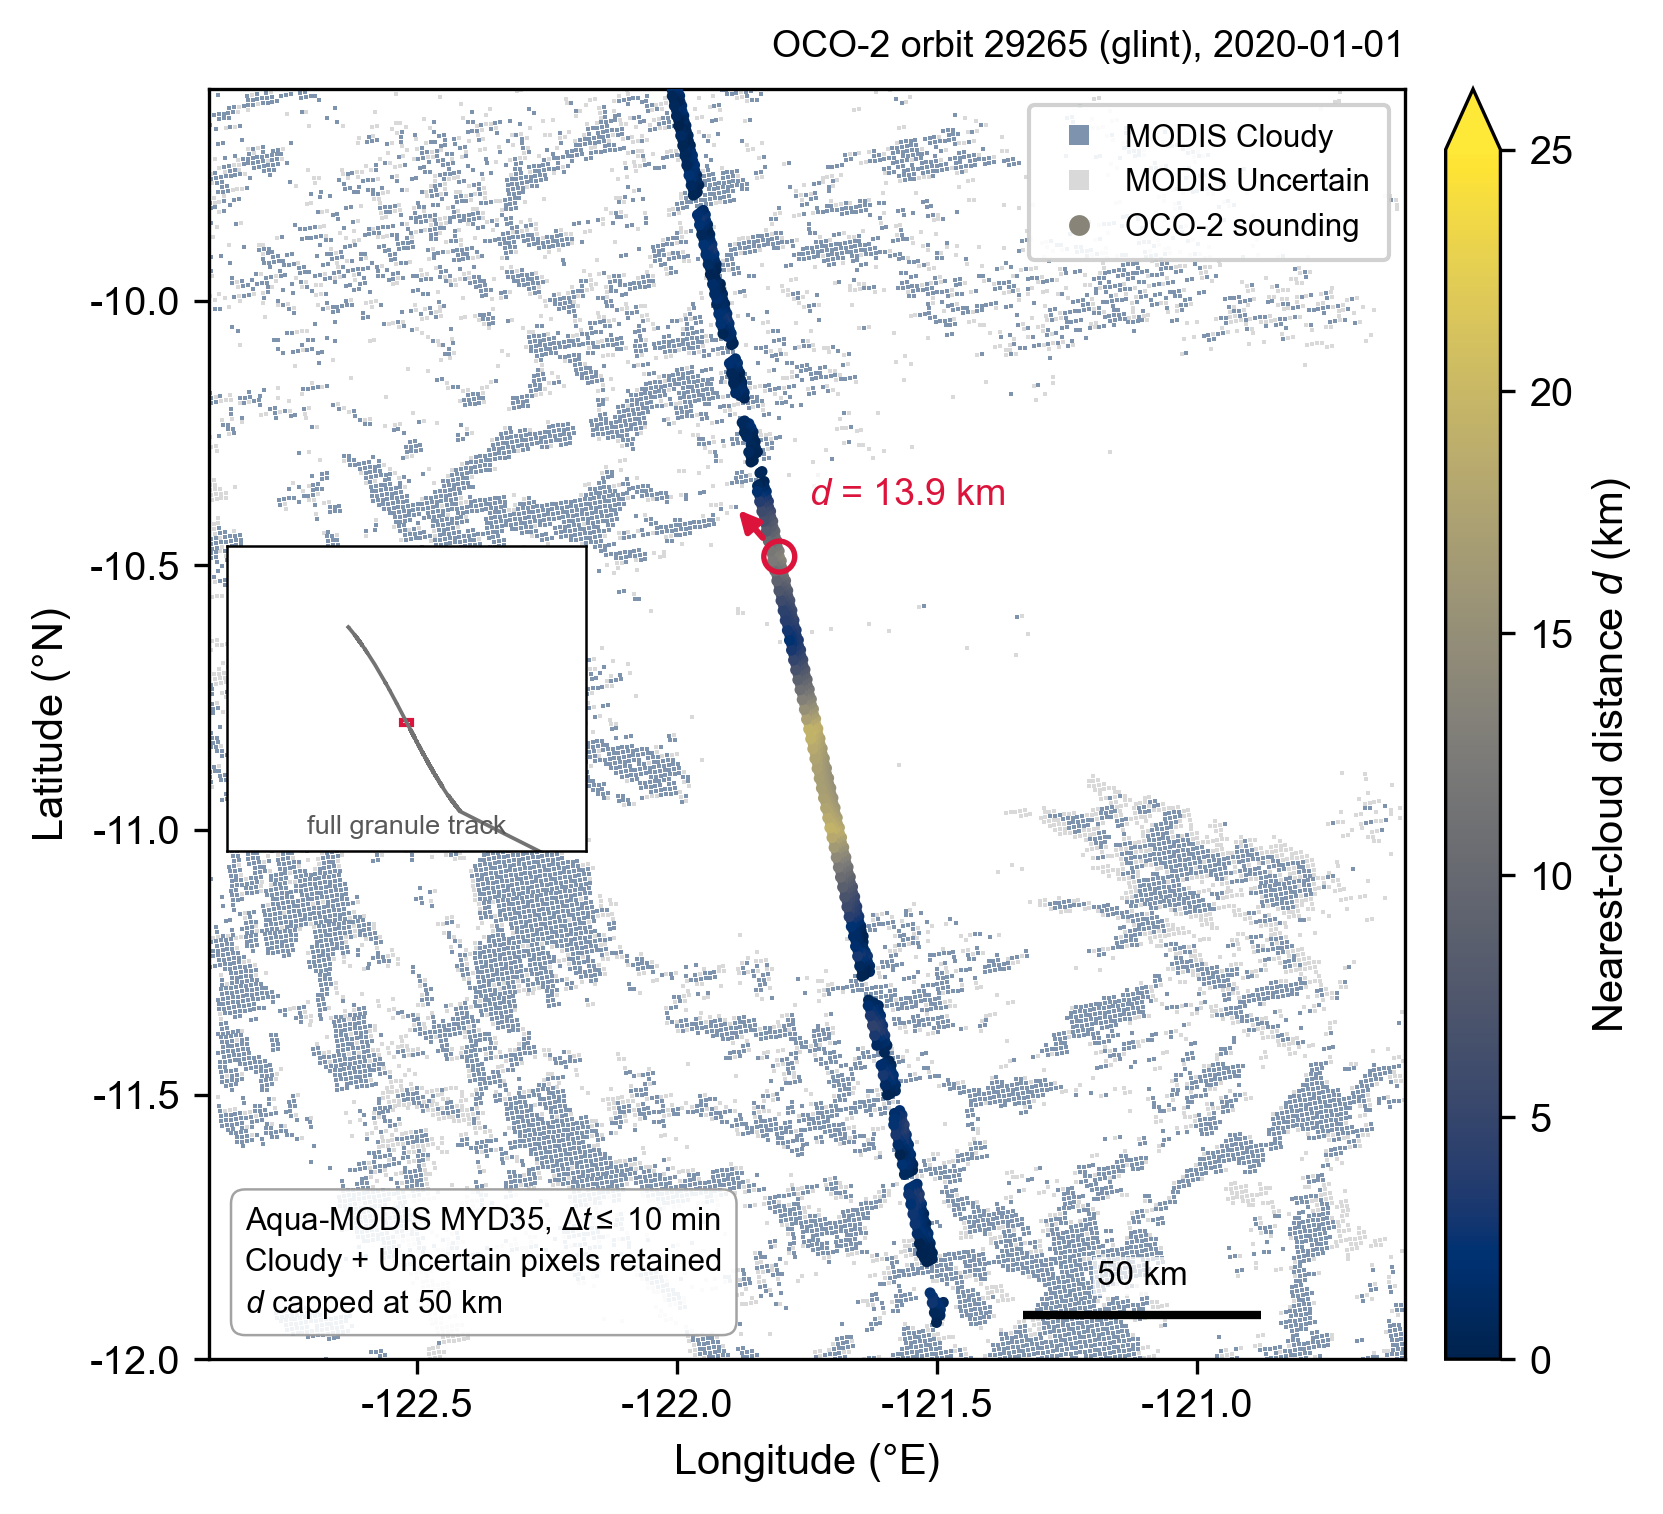
\includegraphics[width=12cm]{figures/fig01_collocation_schematic.png}
\caption{The example of nearest cloud distance result from OCO-2 orbit 29265 on Jan. 1st, 2020.}
\label{fig:OCO-fp-cld_dist}
\end{figure}

\subsubsection{Within-orbit clear-sky anomaly target}

The correction target is an OCO-2-relative $\mathrm{X_{CO2}}$ anomaly that isolates the cloud-proximity signal from the large-scale meridional \ce{CO2} gradient. For sounding $i$, define a local clear-sky reference set from soundings in the same orbit that lie within a latitude half-window $\Delta\varphi$ of $i$ and are far from cloud,
%
\begin{equation}
  \mathcal{R}_i(d_0)
  = \bigl\{\, j :\ |\varphi_j - \varphi_i| \le \Delta\varphi,\
  d_j > d_0,\ \mathrm{X_{CO2,j}}^{\mathrm{B11}}\ \text{valid} \,\bigr\},
  \label{eq:reference-set}
\end{equation}
%
with clear-sky threshold $d_0$ and window $\Delta\varphi = 0.25^{\circ}$. Let
$\mu_i$ and $\sigma_i$ be the mean and standard deviation of the
bias-corrected $\mathrm{X_{CO2,j}}^{\mathrm{B11}}$ over $\mathcal{R}_i(d_0)$. The target is the departure of each sounding from its local clear-sky background,
%
\begin{equation}
  \Delta \mathrm{X_{CO2,i}}^{\mathrm{B11}}
  = \mathrm{X_{CO2,i}}^{\mathrm{B11}} - \mu_i,
  \qquad
  \mu_i = \frac{1}{|\mathcal{R}_i|}
  \sum_{j\in\mathcal{R}_i} \mathrm{X_{CO2,i}}^{\mathrm{B11}},
  \label{eq:anomaly-target}
\end{equation}
%
and is defined only where the reference background is both well populated and
stable,
%
\begin{equation}
  |\mathcal{R}_i| \ge n_{\min} = 5,
  \qquad
  \sigma_i \le \sigma_{\max} = 1.0\ \mathrm{ppm}.
  \label{eq:anomaly-guards}
\end{equation}
%
The population guard $n_{\min}$ suppresses noisy small-sample means, and the
spread guard $\sigma_{\max}$ discards windows where an unresolved
synoptic-scale gradient or residual contamination inflates the reference scatter, or emission sources affect part of footprints in the reference. Soundings failing either test carry no target and are dropped from
training and target-space evaluation.

The clear-sky threshold $d_0$ is the one target parameter. We first use $d_0 = 10$~km to identify the effective cloud-influence distance, and then vary the thresholds by surface: $d_0 = 15$~km over land
(\emph{r15}) and $d_0 = 5$~km over ocean (\emph{r05}), reflecting the different
distance scales at which the land and ocean anomaly--distance curves flatten
(Sect.~\ref{sec:result-cld_dist}). 

We state the principal limitation of this construction at the outset:
Eq.~\eqref{eq:anomaly-target} defines an \emph{OCO-2-relative} anomaly, not an
absolute $\mathrm{X_{CO2}}$ error. The reference mean $\mu_i$ is itself an OCO-2 product and can absorb a genuine within-window atmospheric gradient, so
$\Delta \mathrm{X_{CO2}^{B11}}$ may contain real \ce{CO2} structure in addition to the cloud-induced bias. The stability guard $\sigma_{\max}$ bounds, but does not eliminate, this contamination. Independent validation against TCCON, aircraft, and shipborne references (Sect.~4.5, 4.7) is therefore essential, because it does not rely on the OCO-2-relative target.
